
%%%%%%%%%%

%\begin{frame}{\vskip -0.2cm \large The optimization problem behind classification trees}
\begin{frame}{\vskip -0.4cm \large Le probl\`eme d'optimisation derri\`ere les arbres de classification}

\large
\begin{itemize}
\item
	{\Large Domaine de la fonction objective} {\scriptsize(c.-\`a-d. classe d'hypoth\`eses)}
	{\scriptsize\begin{equation*}
	\left\{\begin{array}{c}
		\overset{{\color{white}.}}{\textnormal{arbres binaires}} \\
		\textnormal{r\'ecursifs}
	\end{array}\right\}
	\quad\sim\quad
	\left\{\begin{array}{c}
		\overset{{\color{white}.}}{\textnormal{fonctions constantes par morceaux}} \\
		\textnormal{resultantes de} \\
		\textnormal{partitionnement binaire r\'ecursif}
	\end{array}\right\}
	\end{equation*}}

	\begin{center}
	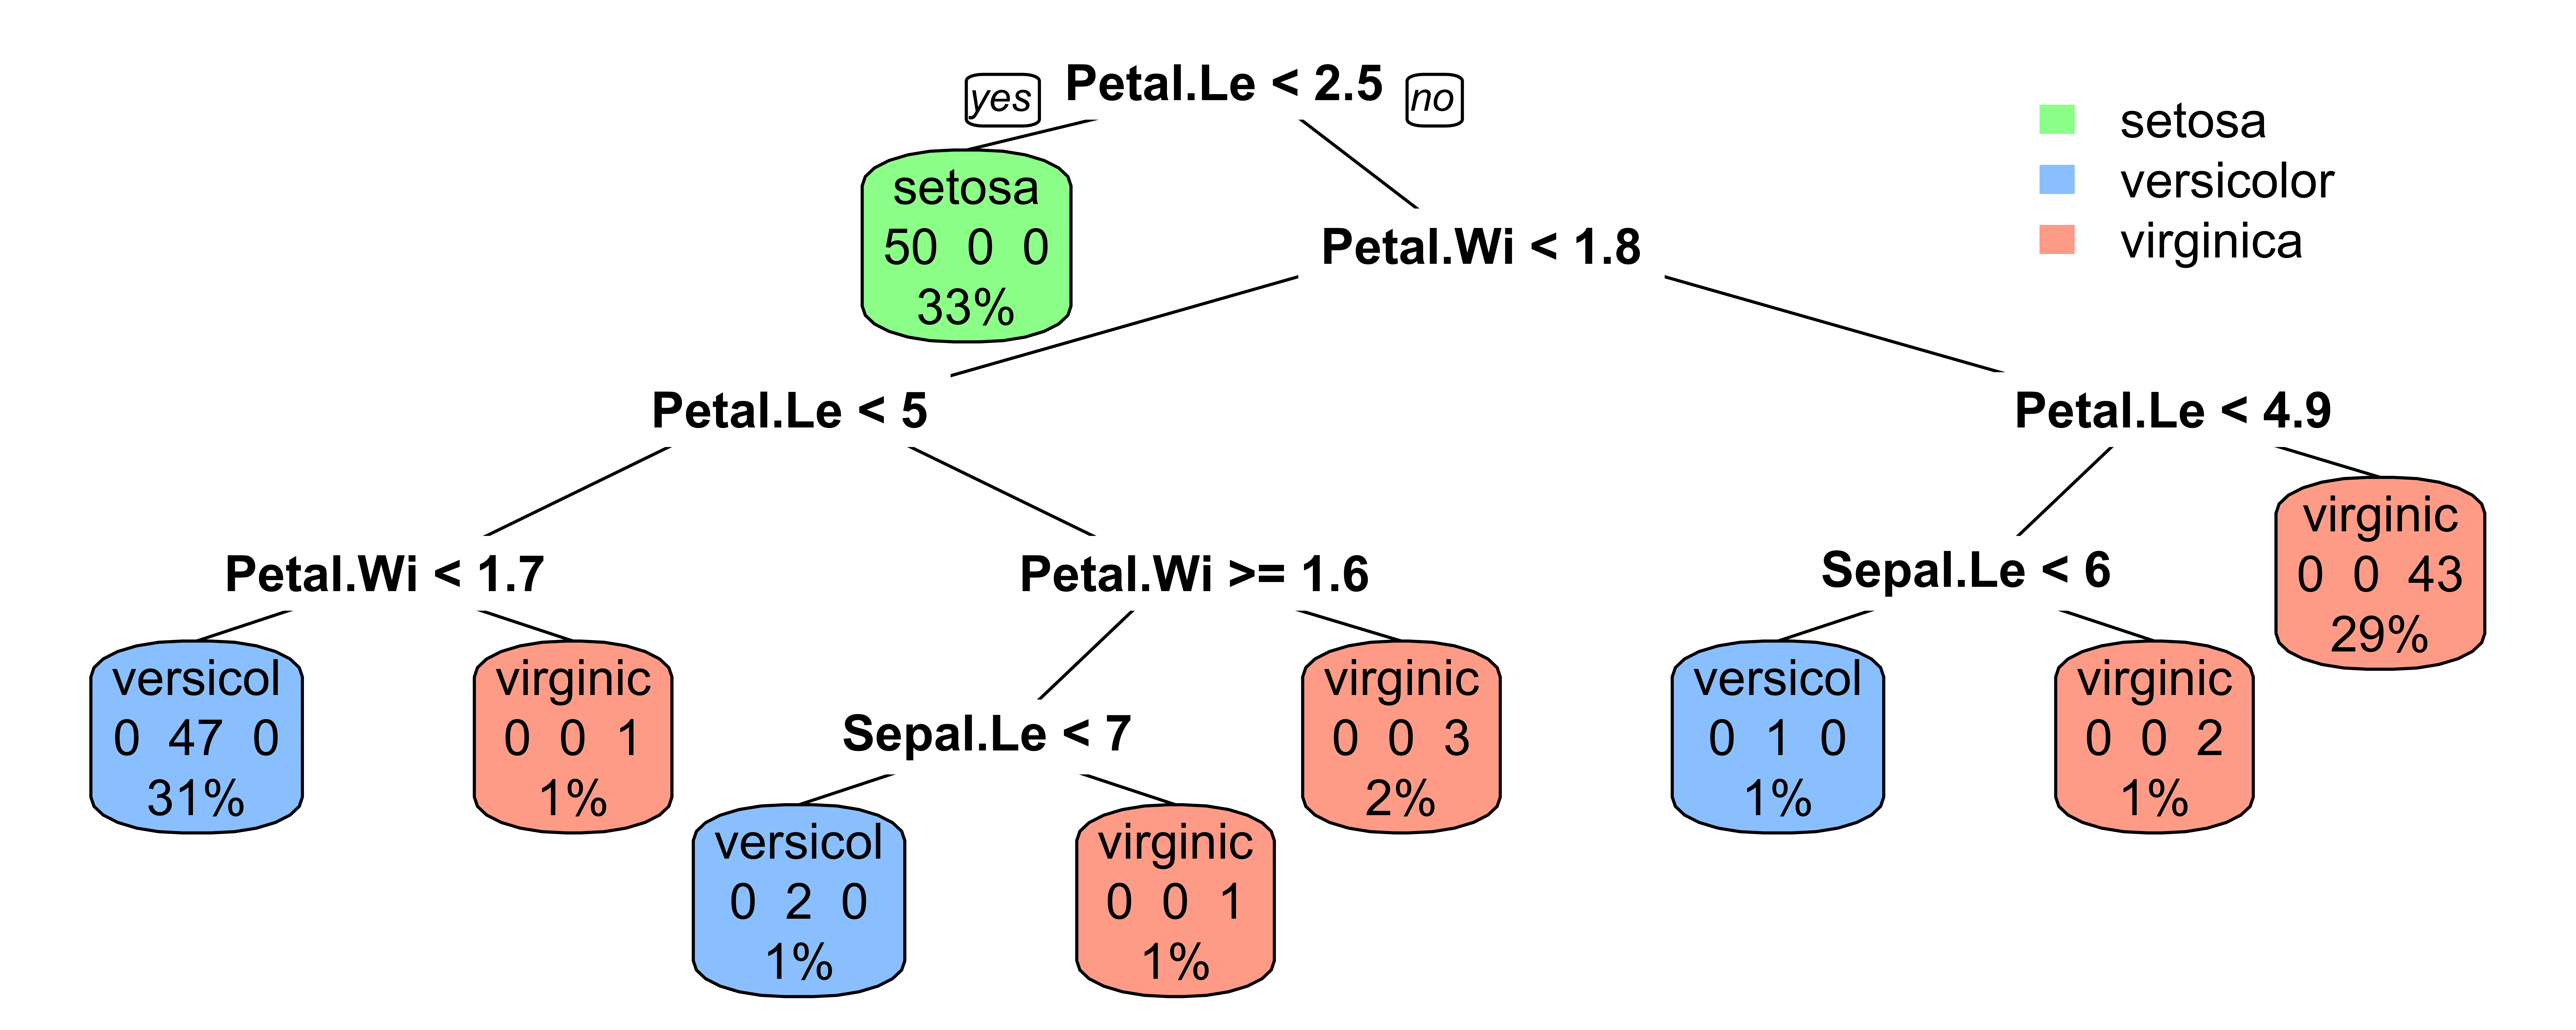
\includegraphics[width=2.5cm,height=3.5cm]{graphics/plot-rpart.png}
	\quad\quad\quad\quad\;\;
	\includegraphics[width=2.5cm,height=3.25cm]{graphics/plot-regression-surface.png}
	\;\;{\color{white}1}
	\end{center}
\end{itemize}


\end{frame}
\normalsize

%%%%%%%%%%
